% -----------------------------------------------
% Template for ISMIR 2010
% (based on earlier ISMIR templates)
% -----------------------------------------------

\documentclass{article}
\usepackage{ismir2010,amsmath,cite}
\usepackage{graphicx}
\usepackage{url}
\usepackage{algorithm,algorithmic}

% added by tbm
\usepackage{subfloat,subfig}
\setlength{\abovecaptionskip}{-3pt}
\setlength{\belowcaptionskip}{10pt} 


% Title.
% ------
\title{Large-scale harmonic patterns clustering}

% Single address
% To use with only one author or several with the same address
% ---------------
%\oneauthor
% {Names should be omitted for double-blind reviewing}
% {Affiliations should be omitted for double-blind reviewing}

% Two addresses
% --------------
%\twoauthors
%  {First author} {School \\ Department}
%  {Second author} {Company \\ Address}

% Three addresses
% --------------
\threeauthors
  {First author} {Affiliation1 \\ {\tt author1@ismir.edu}}
  {Second author} {\bf Retain these fake authors in\\\bf submission to preserve the formatting}
  {Third author} {Affiliation3 \\ {\tt author3@ismir.edu}}
% what order do we use? Thierry, Ron, Dan?  Dan, Thierry, Ron?


\begin{document}
%
\maketitle
%
\begin{abstract}
The goal is to analyze very large collections of music. We describe
a clustering scheme of harmonic patterns that scales linearly in time
with the number of songs analyzed. These harmonic patterns are related
to the \textit{Shingles} idea, but we scale to larger sets and we do not
perform $k$-nn with them. We create a codebook and assert
its properties. In particular, we show that clustering with notions of
bars and song segments helps, and that we get codes associated more
with some artists than others.
\end{abstract}
%
\section{Introduction}\label{sec:introduction}

Large-scale \cite{Bertin-Mahieux2008}. See previous work for \textit{Shingles}
papers.

\subsection{Definitions}
A pattern, or a patch, is a \textit{Shingle} taken from an actual song.
A code is similar to a pattern, but is the result of the clustering
algorithm and most likely does not come from an actual song.
Distortion is our measure of distance between a pattern and a code
(or between two patterns, see equation \ref{eq:dist} in Section 
\ref{sec:experiments}).


\section{Previous Work}\label{sec:prevwork}
Our work can be seen as an extension of the \textit{Shingles} idea
described by Casey and Slaney \cite{Casey2006,Casey2007,Casey2008}.
The two main differences are the clustering framework and the use of
beats and bars to select the position of the \textit{Shingles}.

Casey and Slaney \cite{Casey2006} use LSH \cite{Datar2004} to perform
fast approximate nearest neighbor search. Their implementation is E$^2$LSH
\cite{E2LSH}. This package can efficiently handle about $50$K or $100$K
vectors of size $200$. Even with a better implementation, the LSH
model still has some scaling problem. A large portion of the data
must be known to decide how many projections to use, and what guarantee
of finding the nearest neighbor it can provides. Also, we could fix the
number of projections and consider as clusters all the elements that
fall into the same bin. However, this does not give us a centroid, a
typical pattern representing that cluster.


\section{Data}\label{sec:data}
In this section we present our use of the Echo Nest features and the
datasets we use for training and testing our model.

\subsection{EchoNest API}
We use the Echo Nest analyze API \cite{EchoNest} throughout this work.
The API gives us a chroma vector (length $12$) for every music event, 
or ``segment'', for any song we upload to their platform. 
We also get an estimate of where the beats and the bars are. Beats span over
multiple segments, and bars span over multiple beats. 
We transform the chroma vectors per segment into per beat vectors using a 
simple average. We can then stack beat vectors for a number of bars 
(usually 1 or 2). 
We get a fixed-size patch by resampling the number of chroma vectors. Typically,
there are $4$ beats per bar (Figure \ref{fig:barsize}). 
Thus an appropriate pattern size for one bar
is $12$x$4$ or $12$x$8$.

\begin{figure}[htb]
\begin{center}
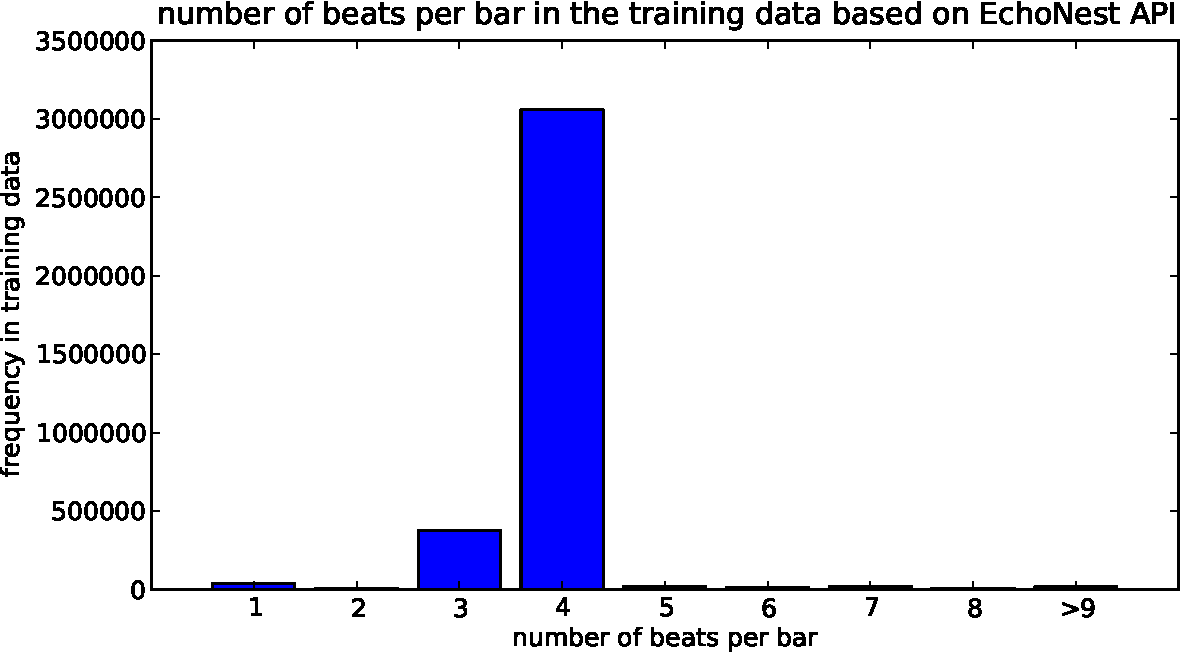
\includegraphics[width=.9\columnwidth]{bar_size_freq}
\end{center}
\caption{\small{
Frequency of the different bar size in the training data.
}}
\label{fig:barsize}
\end{figure}

Note that we do not claim that any of these informations (segments, beats, bars)
are perfectly accurate (e.g. in \cite{Barrington2009a} authors obtain a better
song segmentation than Echonest). Practise showed us that they are reasonable, 
and the size of the data set should make up for the imperfections or noise.
We also believe that patches sizes based on a number of beats or bars are more
meaningful than an arbitrary time length. More on this in the experiments
(Section \ref{sec:experiments} TO BE CHECKED).

\begin{figure}[htb]
\begin{center}
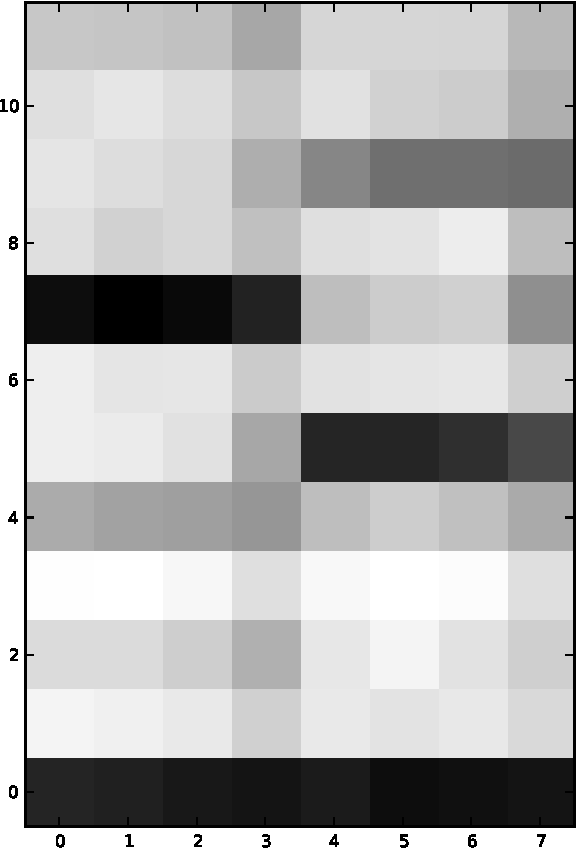
\includegraphics[width=.8\columnwidth]{code}
\end{center}
\caption{\small{A typical code from a codebook of size $200$. 
Patterns represented
$2$ bars and the pattern length was set to $16$.
BLACK AND WHITE VERSION COMING.
}}
\label{fig:code}
\end{figure}

\subsection{Cowbell Dataset}
We have $43,300$ songs, giving  $3,720,091$ non zero bars, a bar usually 
contains $4$ beats. WHERE DOES THIS DATA COMES FROM? GIFT FROM EN?

\subsection{USPOP}
We had acces to a low quality (32kbps) version of the songs in the uspop 2002 
data set \cite{uspop2002}.
This well-known data show a great diversity of pop songs, but is not particular
otherwise. We also tried to use Tzanetakis dataset \cite{Tzanetakis2002a}, but 
the $30$ seconds segments seemed hard to analyze by the Echo Nest API, most did
not contain any bar.

uspop2002 serves as testing set to measure how well a codebook learned on
the Cowbell data set can represent new songs. We get Echo Nest features
for $8651$ songs from that dataset.

\subsection{Artist Set}
A set of songs from $20$ artists.


\section{Algorithm}\label{sec:algo}
In this section we present the creation of the harmonic patterns from
the Echo Nest data. Then, we explain the online vector quantization algorithm
used to learn a codebook of those patterns.

\subsection{Pattern Creation}
Here we should explain key invariance, resizing, etc, and not in the
experiment section.

We try to normalize the patterns in respect to the key. We roll the matrix
so the row with the more energy is always the lowest one. This can easily be
seen in Figure \ref{fig:code}. We considered the same technique for rolling
along the other axis and be invariant regarding the downbeat. However, it
seems less robust to noise. Note that we roll each pattern independentely.
Also, this implies that the pitch envelope is important rather than the actual 
pitches.


\subsection{Codebook Learning}
We use an online version of the vector quantization algorithm 
\cite{Gersho1991}. This can also be seen as an online K-means.
The idea is as follow: take a sample from your data, find the closest
code in the codebook, bring that code closer to the sample by some amount.
The details are explained in Algorithm \ref{algo:vq}. Note that this
algorithm, though not optimal, is $O(n)$ with $n$ number of songs seen.
Thus it scales linearly to any size of data set. The setting of the learning
rate might become trickier, but this is not fundamentally a problem.

We initialize the codebook by choosing $K$ random points from our dataset.


\begin{algorithm}
%\caption{Pseudocode of Vector Quantization}
\begin{algorithmic}
\STATE$l$ learning rate
\STATE$\{P_n\}$ set of patches
\STATE$\{C_k\}$ codebook of $K$ codes
%\STATE $m \leftarrow b$
\REQUIRE $0 < l \leq 1$
\FOR{$nIters$}
\FOR{$p \in \{P_n\}$}
\STATE$c \leftarrow min_{c \in C_k} dist(p,c)$
\STATE$c \leftarrow c + (p - c) * l$
\ENDFOR
\ENDFOR
\RETURN $\{C_k\}$
\caption{\small{Pseudocode of Online Vector Quantization. Note that we can 
replace the number of iteration by a threshold on the distortion over some 
test set.}
\label{algo:vq}}
\end{algorithmic}
\end{algorithm}



\section{Experiments - Fundamentals}\label{sec:experiments}
In this section we assert the basic properties of our encoding scheme.
The first subsection gives the details to reproduce the experiments,
such as the distance measure and learning rate. In the second subsection, we
measure properties such as ``how the number of codes affect the distortion''
and ``how many learning samples should we use''. Though important numbers
to report, the busy reader could skip to subsection \ref{ssec:random}
and the following sections.
Note that we will present two additional experiments in 
Section \ref{sec:exps2}.


\subsection{Setting}\label{ssec:setting}
We take one or two bars, normalize the patches to size 4, 8, or 16.
We roll the patch to be invariant to the key (on the patch level, not on
the song level). We learn a codebook of size $K$ over the cowbell dataset 
using the VQ algorithm (Algorithm \ref{algo:vq}). A typical learning rate 
is $0.01$ for $200$ iterations over the whole dataset.

We use the codebook to encode our testing set (see Section \ref{sec:data}).
Each pattern is encoded with only one code. We can measure the average
distance between a pattern and its encoding. We can also measure the use
of the different codes, i.e. the size of the cluster around a code.

As a distance measure (or distortion measure) between patterns, we use
the average squared euclidean distance. In details, if a pattern $p1$
is composed of elements $p1_{i,j}$, and similarly for a pattern $p2$,
the distance between $p1$ and $p2$ is:
\begin{eqnarray}
  dist(p1,p2) = \sum_{i,j} (p1_{i,j} - p2_{i,j})^2 / size(p1)  \label{eq:dist}
\end{eqnarray}
We assume $p1$ and $p2$ have the same size.


\subsection{Basic Properties}
This section present some fundamental results of the clustering algorithm.
These are important, but do not change the larger picture. Thus we will not
spend too much time describing them. In short: more training samples is
better, more codes is better, larger patterns are more difficult.
\begin{itemize}
\item First, a larger dataset gives a better encoding codebook. See Figure
\ref{fig:data_sizes}.
\item Secondly, a larger codebook better encodes new song. See 
Table \ref{tab:cbsize}.
\item Finally, larger patterns are more difficult to encode, thus require
larger codebooks. See Figure \ref{fig:perbeat}.
\end{itemize}

These properties are important to verify and measure, but they are not
surprising for a clustering algorithm. We move on to more interestng facts.

\begin{figure}[htb]
\begin{center}
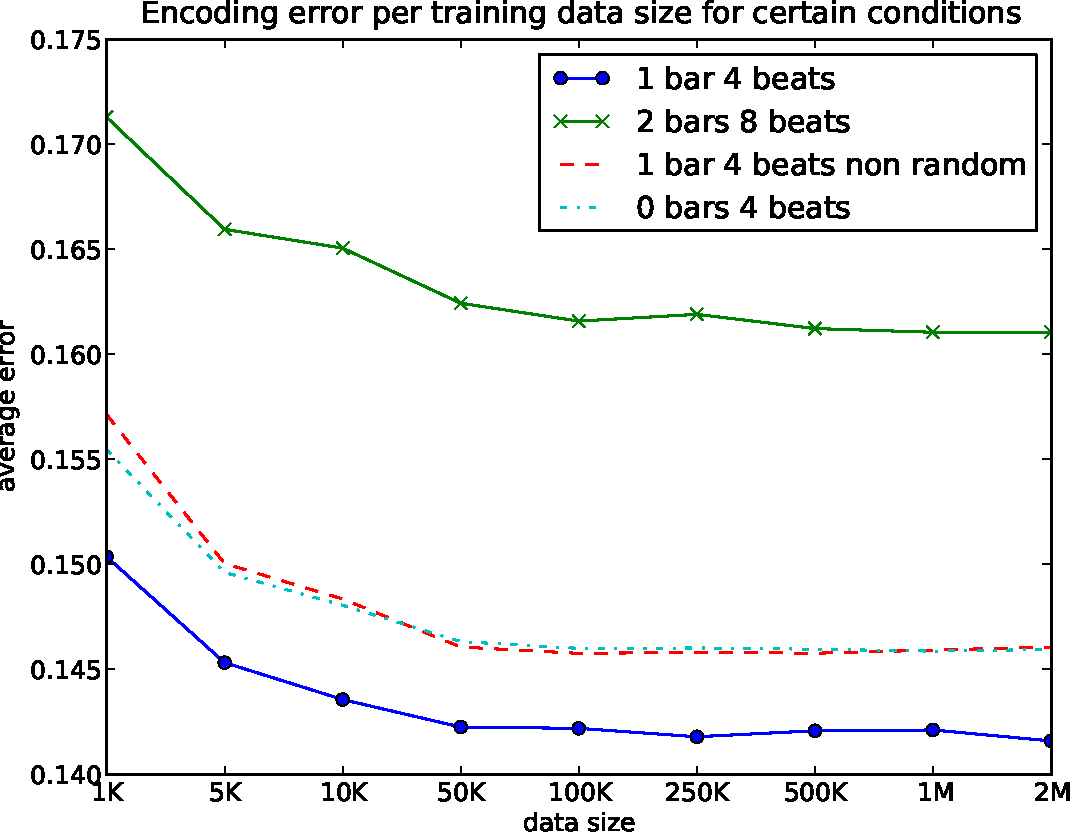
\includegraphics[width=.99\columnwidth]{data_sizes}
\end{center}
\caption{\small{Distortion for a codebook of size $100$ encoding one bar
at a time, a bar being represented by $4$ chroma feature vector.
Therefore, a code or a pattern is of size $12$ x $4$ = $48$.
Distortion measure on the test data set. Data size tested range
from $10$ thousands to $2$ millions. Patterns were selected at
random from the dataset of approximately $3,7$ million patterns.
OLD GRAPH WITH OLD NUMBERS
}}
\label{fig:data_sizes}
\end{figure}

% NEW RESULTS COMING SOON WITH FIXED SIZED DATASET
\begin{table}
\begin{center}
\begin{tabular}{|l|l|c|}
\hline
\# codes & \# samples & avg. dist \\ \hline \hline
1 & $500$ & $0.066079$ \\
10 & $5$K & $0.045690$ \\
50 & $25$K & $0.038456$ \\
100 & $50$K & $0.036725$ \\
200 & $100$K & $0.033923$ \\
500 & $250$K & $0.030973$ \\
1000 & $500$K & \\ \hline
\end{tabular}
\end{center}
\caption{\small{Experiment with the codebook size. We train on patterns
corresponding to $1$ bar resized to $4$ beats. The number of training
samples is set to $500$ times the number of codes. 
NEW RESULTS COMING SOON WITH FIXED SIZED DATASET }}
\label{tab:cbsize}
\end{table}


\begin{figure}[htb]
\begin{center}
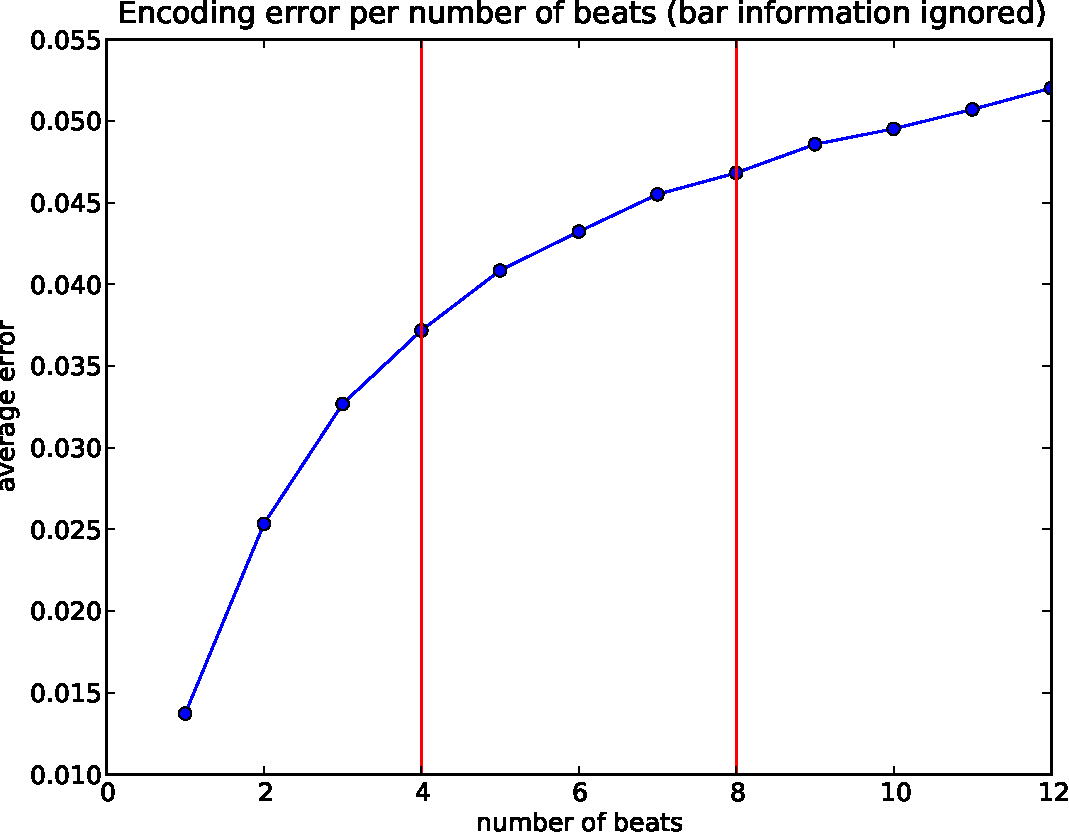
\includegraphics[width=.9\columnwidth]{encoding_per_beat}
\end{center}
\caption{\small{Encoding larger and larger patterns with a fixed size
codebook.}}
\label{fig:perbeat}
\end{figure}

\subsection{Music Randomness}\label{ssec:random}
It will not surprise any reader, music is not random. This fact should
become apparent in our experiments in the following way. Information
theory tells us that if the signal to encode doubles, we need to square
the size of the codebook to encode it with the same distortion.

To help the intuition, here is an example. Imagine a binary array of 
length $1$. We need two
codes to encode perfectly: $(0)$ and $(1)$. If the binary array is now of
length $2$, we now need four codes: $(0,0)$, $(0,1)$, $(1,1)$ and $(1,0)$.

Since music is not random, we expect that squaring the codebook when the
pattern size doubles will rather give improved results than constant ones.
See Figure \ref{fig:size_pattern}.

% see generate_expo_codes_curves.py to generate the following figure:
\begin{figure}[htb]
\begin{center}
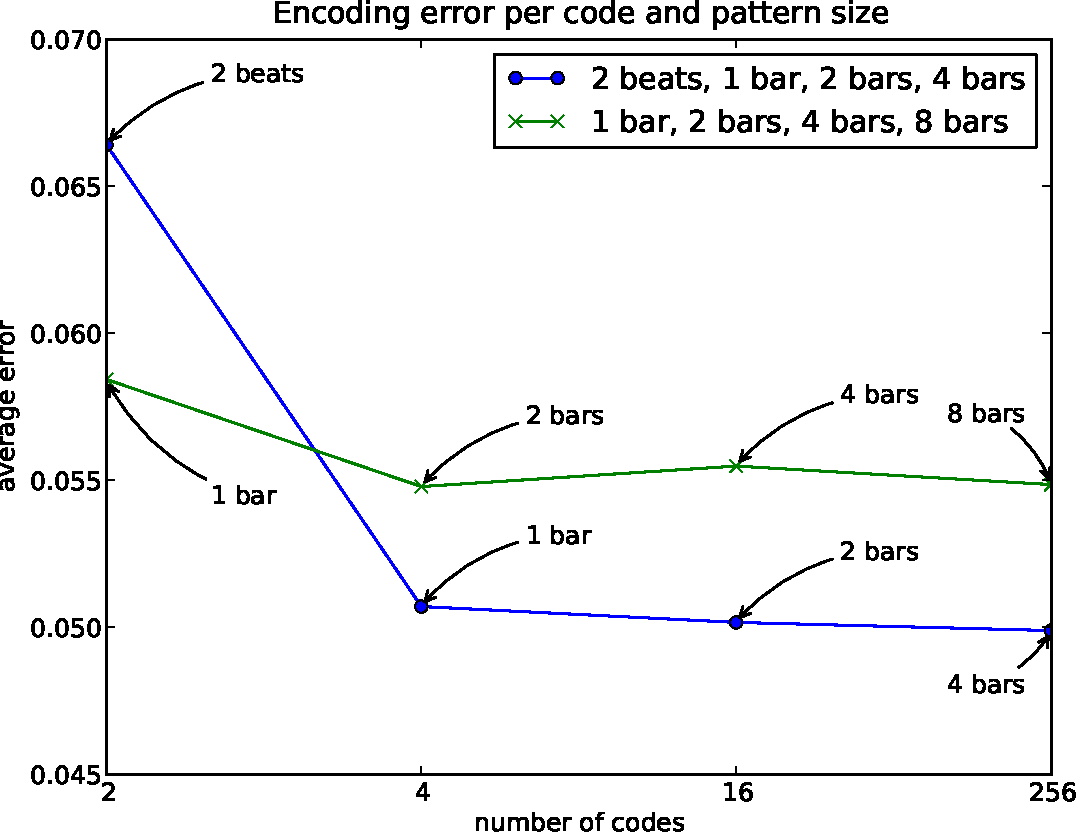
\includegraphics[width=.99\columnwidth]{codesize_patternsize}
\end{center}
\caption{\small{NEW RESULTS COMING IN}}
\label{fig:size_pattern}
\end{figure}

\section{Visualization} \label{sec:visu}
The goal here is to give an intuition to the reader of what kind of
typical patterns do we get. We also want to have a feel for what the
clusters look like, how many boring sustained notes are encoded in the
codebook, can the codebook describes the complexity of the music space, etc.

Below we present some figures to help the reader with those questions.
Please bear in mind the limited space.

\subsection{Encoding of a Song}
Here we present a song with its two encodings. First, the harmonic patterns
given by the EchoNest. Secondly, each pattern is encoded by its closest
code in the codebook. See Figure \ref{fig:encodesong}.

\begin{figure}[htb]
\begin{center}
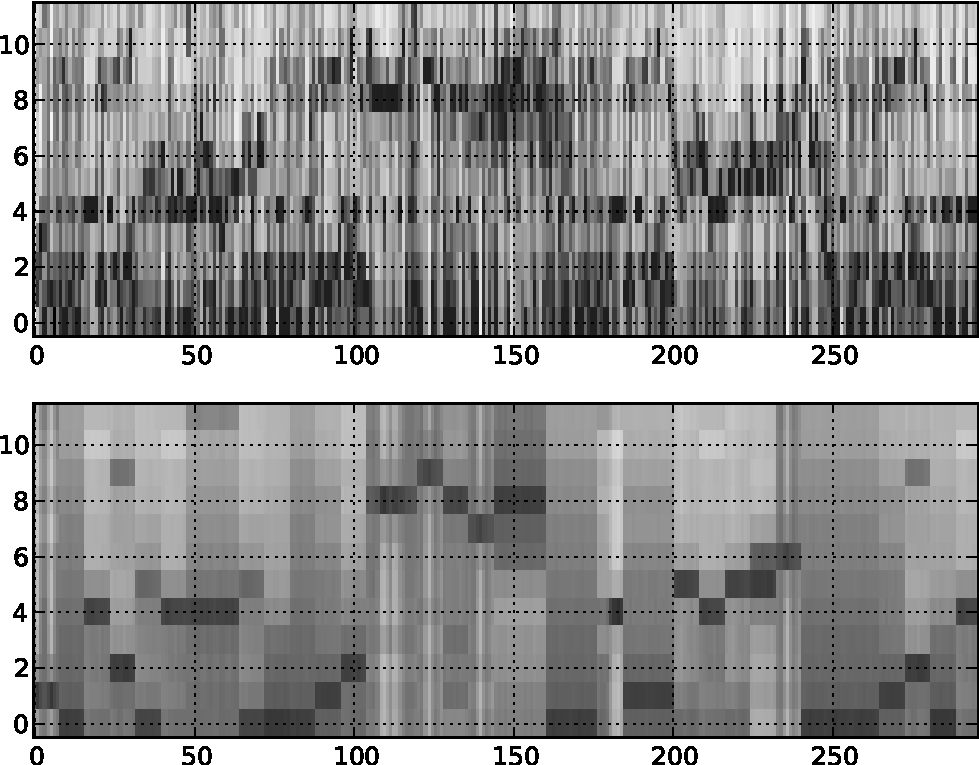
\includegraphics[width=.9\columnwidth]{song_encoded}
\end{center}
\caption{\small{Original song and its encoding. Must get a better one for
the paper!!!!!!}}
\label{fig:encodesong}
\end{figure}

\subsection{Codebook}
We can present the most typical patterns (Figure \ref{fig:codes1}). 
Then, LLE? (Figure \ref{fig:lle}). 
Then, the graph on variance. (Figure \ref{fig:code_var}).

\begin{figure}[htb]
\begin{center}
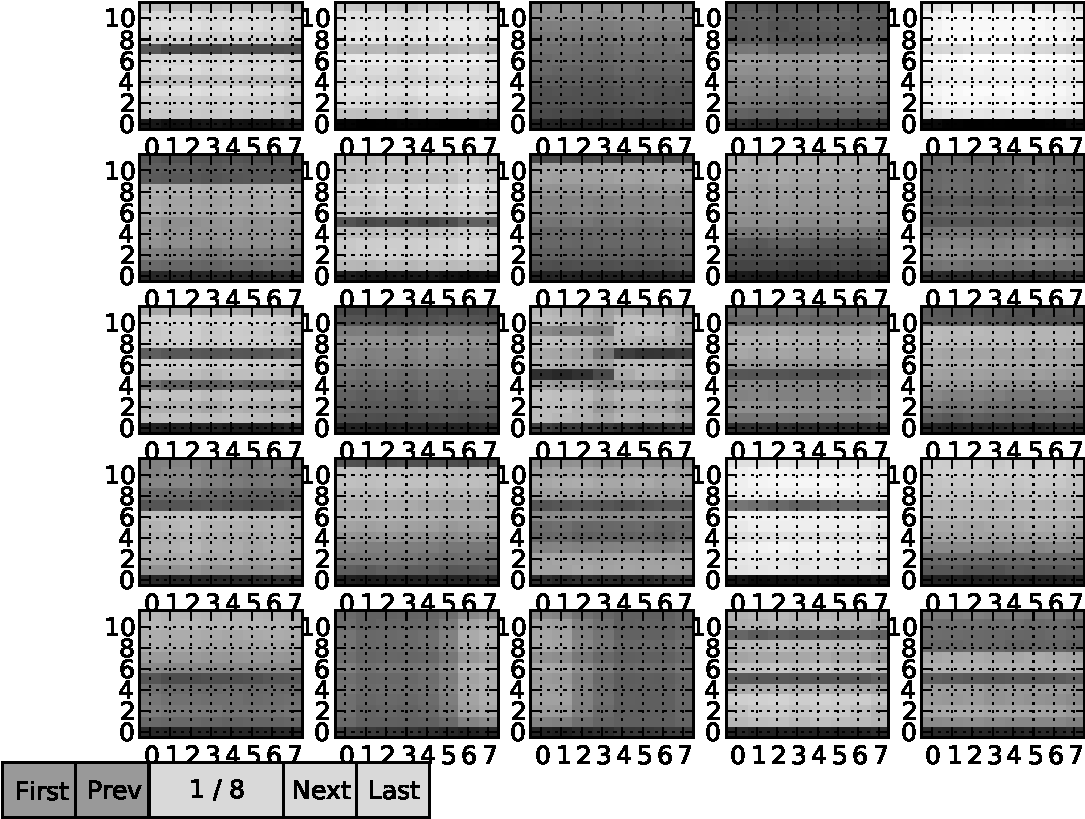
\includegraphics[width=.9\columnwidth]{codes1}
\end{center}
\caption{\small{Most used codes in the codebook.}}
\label{fig:codes1}
\end{figure}

\begin{figure}[htb]
\begin{center}
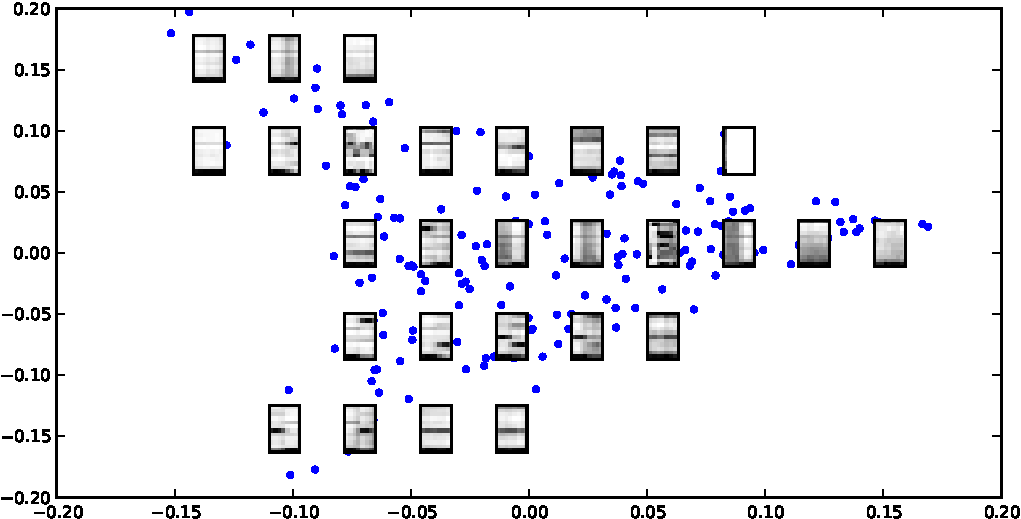
\includegraphics[width=.9\columnwidth]{codes_lle}
\end{center}
\caption{\small{Locally linear embedding (LLE) visualization of the codebook.}}
\label{fig:lle}
\end{figure}

\begin{figure}[htb]
\begin{center}
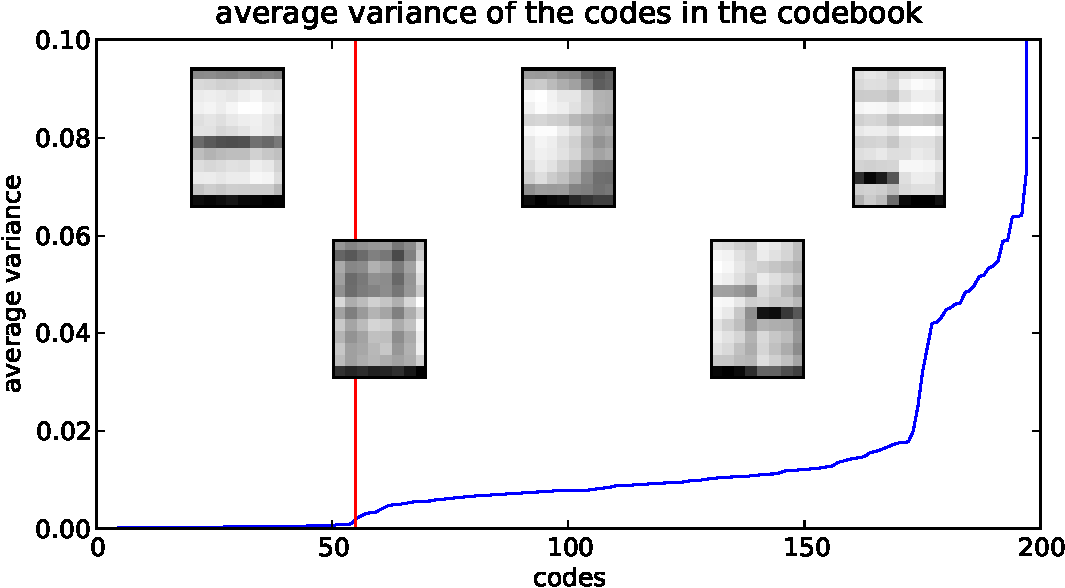
\includegraphics[width=.9\columnwidth]{code_variance}
\end{center}
\caption{\small{Average variance in time of a codebook. The vertical
axis cuts at the $63$rd pattern, a rough estimate of the number of 
sustained note patterns.
}}
\label{fig:code_var}
\end{figure}

\subsection{Cluster}
Here we present real patterns that are closer to the code presented in ...
than any other code. The goal is to feel how much variance is present in
a cluster. See Figure \ref{fig:cluster}.

\begin{figure}[htb]
\begin{center}
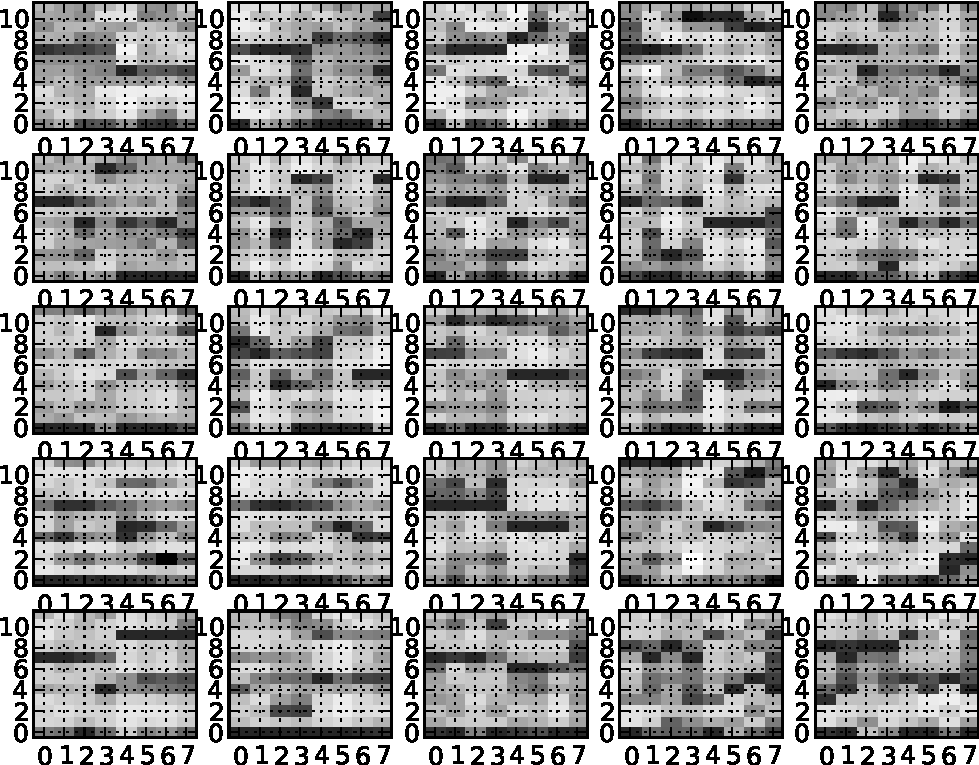
\includegraphics[width=.9\columnwidth]{close_patterns1}
\end{center}
\caption{\small{Cluster around some pattern... TO BE REDONE}}
\label{fig:cluster}
\end{figure}

\section{Further Experiments}\label{sec:exps2}
We have shown the basic properties of our clustering algorithm in
Section \ref{sec:experiments}. In Section \ref{sec:visu}, we showed
how to visualize the codebook and the clusters. We know move on to
show other applications that can take advantage of our clustering.
In the next two subsections, we talk about song segmentation and
artist recognition. Our algorithm was not devised for any of these tasks,
but some information contained in the centroids can be naturally used.

\subsection{Song Segmentation}
We explained that we used bars as defined by the EchoNest algorithm to
train our patterns. Let's assume once again that those bars are
reasonable. We investigate whether we could recover the bar segmentation
of new songs from our codebook. It would helps us assert that codes
encodes something related to bars, for instance a strong beat at the
beginning. Results are shown \ref{tab:offset}. We find the right segment
with an accuracy of $62\%$ where random is $25\%$. Details of the
experiment follow.

We train a codebook of size $100$ on bars resized to $4$ beats. Then,
we take the longest sequence of bars of $4$ beats in the test set.
As we mentioned before, $4$ beats is the most common (by far!) bar size
in terms of beats according to the EchoNest API. We then encode this
sequence using an offset of $0$, $1$, $2$ or $3$ beats. The best offset
is the one that gives the encoding with the lowest distortion. The
good answer is an offset of $0$.

\begin{table}
\begin{center}
\begin{tabular}{c|c}
%\hline
offset & \% of times chosen \\ \hline
0 & $\mathbf{62.6}$\\
1 & $16.5$\\
2 & $09.4$\\
3 & $11.5$\\
\end{tabular}
\end{center}
\caption{\small{
Best offset according to our codebook. The real one is $0$.
}}
\label{tab:offset}
\end{table}

\subsection{Artist Recognition}
Let us be clear, the clustering method proposed in this work is not
intended to perform well at artist recognition. An obvious fact is that
we lose all timbral information which would be usefull. However, we can
imagine that some artist use more often some patterns than others.
Best accuracy reported\footnote{few details given to preserve anonymity} 
is around $54.5\%$. Our result is $23.4\%$. Random
is around $5\%$. The confusion matrix can be seen in Figure \ref{fig:conf_mat}.
Details of the experiment follow.

All songs in the artist dataset are encoded as an histogram of the codes
used in that song. The frequency values are normalized by the number
of patterns in the song. We test each song in a leave-one-out setting.
Leaving aside the test song, we represent the $20$ artists by the average of
the song histograms of that artist. The test song is compared to
the histogram of each artist using euclidean distance.


\begin{figure}[htb]
\begin{center}
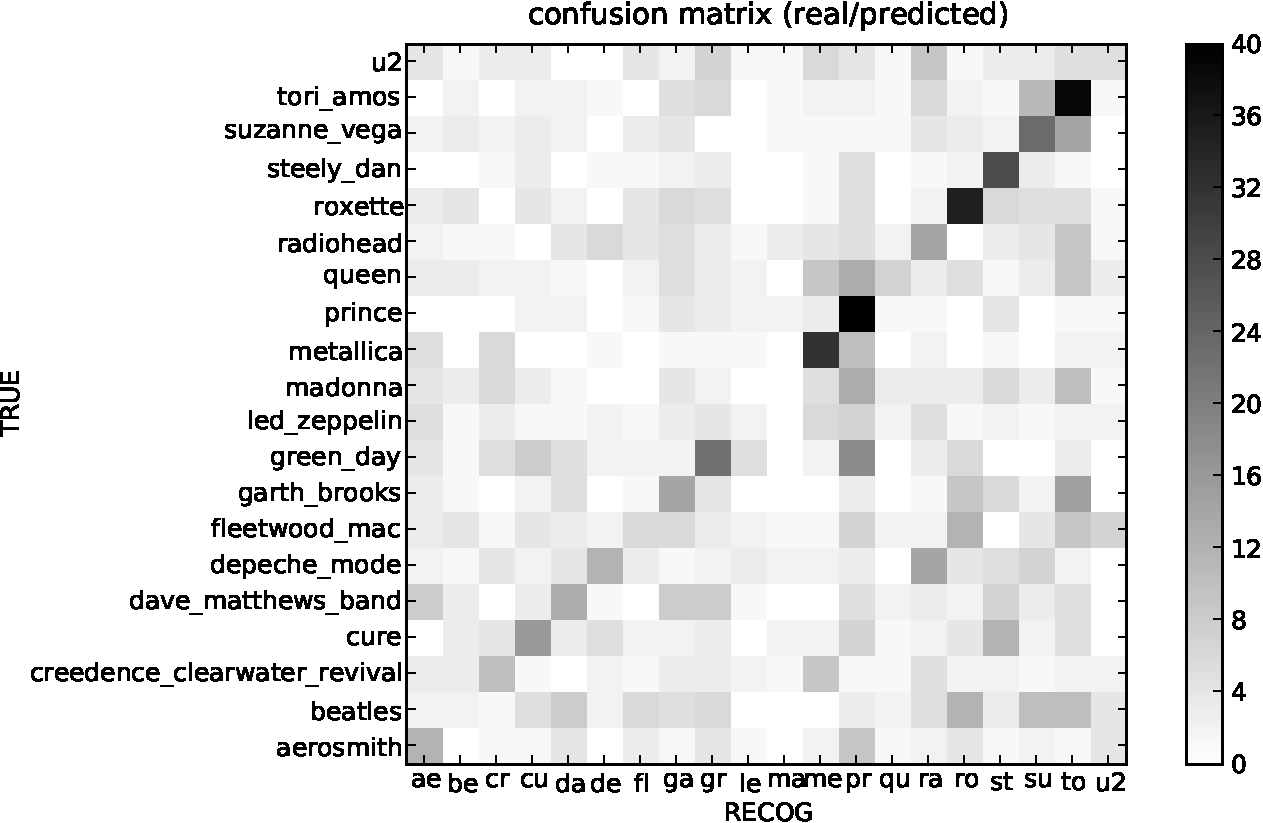
\includegraphics[width=.9\columnwidth]{conf_mat_per_artist}
\end{center}
\caption{\small{Confusion matrix for artist recognition task.}}
\label{fig:conf_mat}
\end{figure}

Looking at the most typical patterns per artist can be insightful.
To find these patters, we compare its use by one artist and divide
by its use by all artists. In Figure \ref{fig:typicalpat} we see 
Metallica's pattern, then Tori Amos and
Suzanne Vega's pattern. These three artists were easily identified.

% ignoring the two following figures
\iffalse
\begin{figure}[htb]
\begin{center}
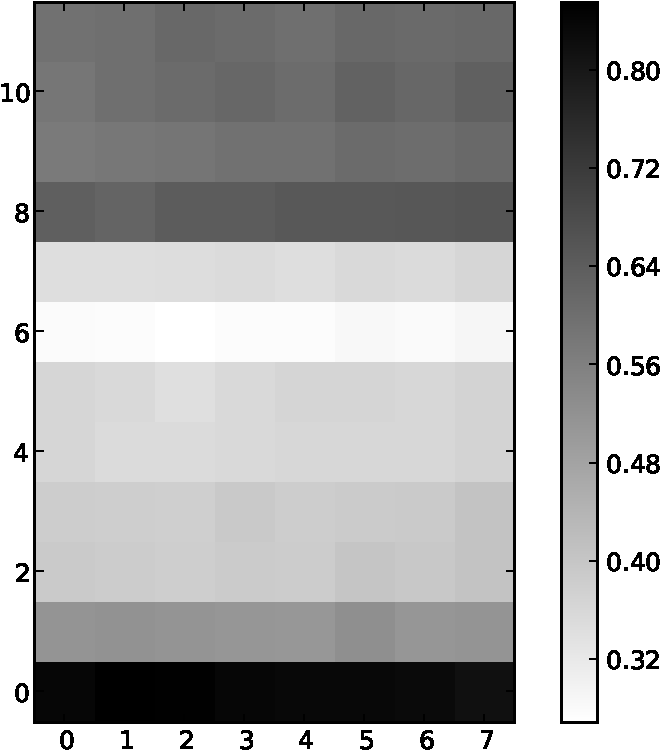
\includegraphics[width=.4\columnwidth]{metallica_pattern}
\end{center}
\caption{\small{Most typical pattern for Metallica.
COULD BE MIXED WITH TORI AMOS FIGURE.
}}
\label{fig:metallica}
\end{figure}

\begin{figure}[htb]
\begin{center}
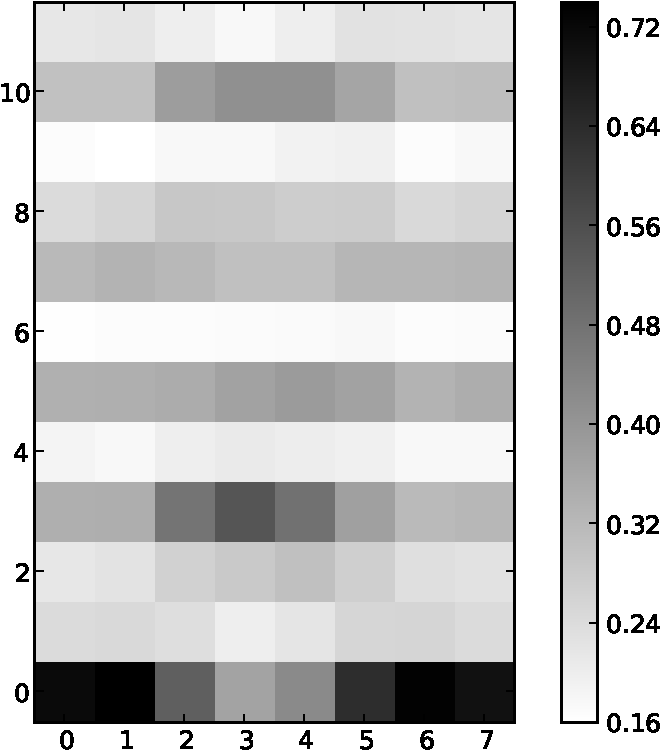
\includegraphics[width=.4\columnwidth]{toriamos_suzannevega_pattern}
\end{center}
\caption{\small{Most typical pattern for Tori Amos and Suzanne Vega.}}
\label{fig:amosvega}
\end{figure}
\fi


\begin{figure}[htb]
  \centering
  \subfloat[][\small{Metallica}]{\label{fig:metallica2}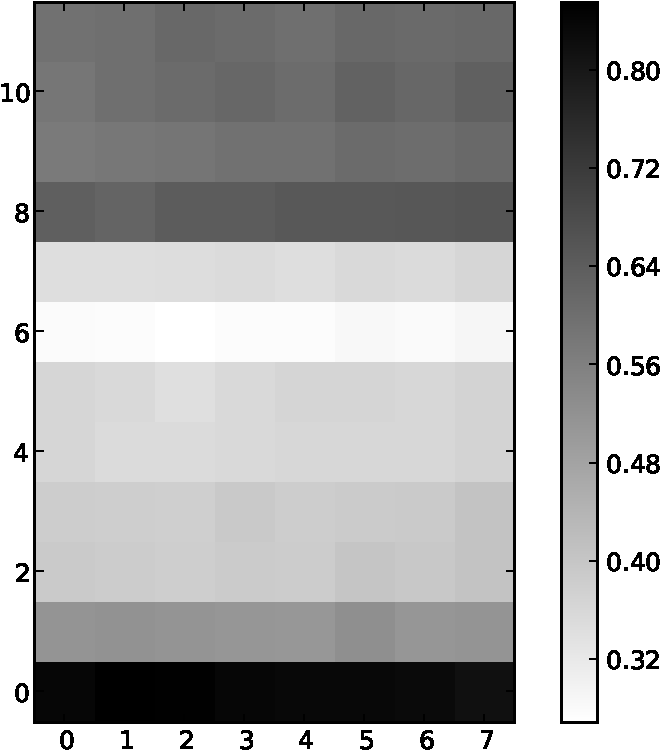
\includegraphics[width=0.4\columnwidth]{metallica_pattern}}                
  \subfloat[][\small{Tori Amos / Suzanne Vega}]{\label{fig:amosvega2}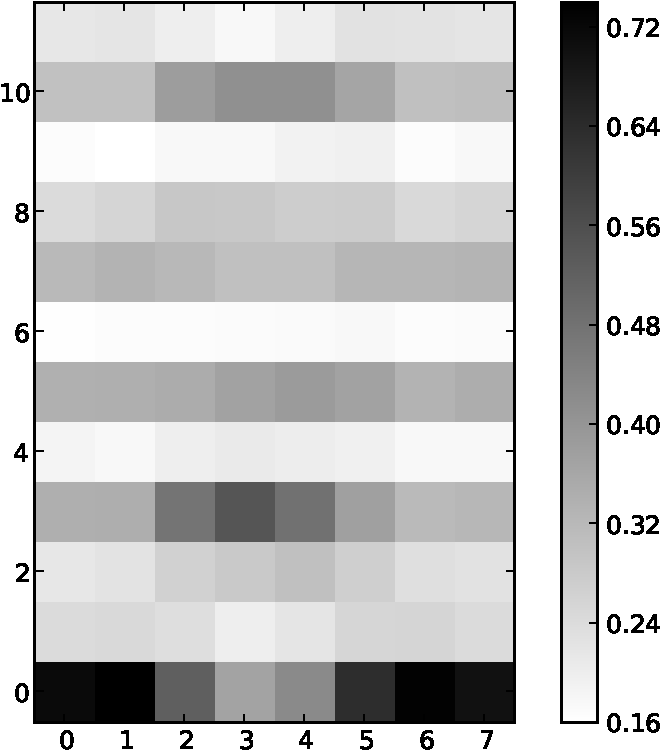
\includegraphics[width=0.4\columnwidth]{toriamos_suzannevega_pattern}}
  \caption{\small{Typical patterns for different artists.}}
  \label{fig:typicalpat}
\end{figure}



\section{Conclusion and Future Work}
We presented a practical method to perform large-scale clustering of
harmonic patterns. We assessed the basic properties of the method through
experiments on a large collection of music. We suggested many ways
to interpret the data through visualization (LLE) and further encoding
(NMF). We discussed the possibility to move to even larger scales
and we provided our source code\footnote{Code not yet released to preserve
submission's anonymity}.

As for enhancements, we specifically did not compress our features using
gaussian mixtures or other generative model. That being said, these methods
could be use to develop better distance measures between \textit{Shingles}.
The use of the euclidean distance is arbitrary. Summarizing patches
with gaussians, and then comparing the distance between those gaussians,
could reduce the influence of the noise in the distance measure.

Moving on to larger scales, we could imagine merging codes together and
splitting some on two if the clusters become too small or too large.We could
also cluster the codebook itself, in a similar fashion as hierarchical
gaussian mixtures \cite{Vasconcelos2001}.


\small
%\section{Acknowledgements}
%Thierry is NSERC graduate fellow, or some title like that.
% Graham for the NMF stuff, unless is an author.

%\begin{thebibliography}{citations}
%\bibitem{Someone:04} 
%X. Someone and Y. Someone:
%{\it Title of the Book},
%Editorial Acme, Utrecht, 2004.
%\end{thebibliography}

\bibliography{tbm_bib}





\end{document}
